\iffalse
\subsection{Guide Robot}
In Japan, a robot has been designed to guide in a shopping mall. It can guide customers by gesture, such as pointing in the direction of where to go and using speech saying e.g. "Please go that way", followed by further instructions such as "...then turn left" or "...then turn right" if needed. The robot can also recommend stores or restaurants if the customer has not decided where to go, by asking questions and using the conversation to choose a store or restaurant fitting the customer's answers\cite{GuideRobotShopping}.

\begin{figure}[H]
    \begin{minipage}[b]{0.5\linewidth}
        The robot has sensors to enable position estimation, person identification and speech recognition. Using floor sensors, it can estimate the position and identify the position of multiple people. For identifying the people, a passive-type radio frequency identification tag. For speech recognition a human operator helped alongside the robot, since the robot only had 21.3\% word accuracy of speech recognition in a real environment\cite{GuideRobotShopping}. The whole setup can be seen in fig. \ref{fig:guide_robot}.
    \end{minipage}
    \hspace{0.4cm}
    \begin{minipage}[b]{0.45\linewidth}
        \centering
        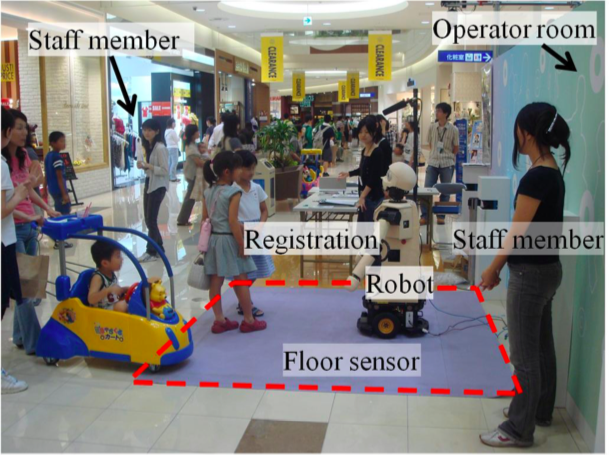
\includegraphics[width=\textwidth]{figures/robot_shoppingMall.png}
        \caption{Setup of the guidance robot\cite{GuideRobotShopping}}
        \label{fig:guide_robot}
    \end{minipage}
\end{figure}
The robot can have a relatively advanced conversation with the customer. As mentioned earlier, the robot can recommend places by asking the customer a few questions regarding the possible results. Additionally, it has the ability to change friendliness in behaviour. If a customer has repeatedly visited the robot, it gradually changes its behaviour from first say "I'm a little nervous talking with you for the first time" to "I think we are friends".\\

For people-identification, they have used a radio-frequency identification (RFID) tag. It is not needed to have a RFID tag to interact with the robot, but the conversation will be more personalised. The robot will start by greeting the customer by name and the recommendations will be suited to the specific customers earlier preferences. If the customer does not have an RFID tag, the robot will provide a more simple interaction providing shopping information and route guidance.\\
The robot is implemented with a gaze behaviour, which is the robot will look at the face of the customer interacting with it. This is done by typing in the height of the customer in the RFID tag, so the robot orient its gaze to the direction and estimated height of the face\cite{GuideRobotShopping}.
\fi